\documentclass{beamer}
\usepackage{ctex, hyperref}
\usepackage[T1]{fontenc}

\usepackage{latexsym,amsmath,xcolor,multicol,booktabs,calligra}
\usepackage{graphicx,pstricks,listings,stackengine}
\usepackage{subcaption}

\author{李睿潇、朱元依、张政镒、李少群}
\title{AzureMIPS——顺序双发射11级流水处理器}
\subtitle{NSCSCC2022 决赛答辩}
\institute{复旦大学}
\date{2022年8月20日}
\usepackage{Tsinghua_fdublue}

\def\cmd#1{\texttt{\color{red}\footnotesize $\backslash$#1}}
\def\env#1{\texttt{\color{blue}\footnotesize #1}}
\definecolor{deepblue}{rgb}{0,0,0.5}
\definecolor{deepred}{rgb}{0.6,0,0}
\definecolor{deepgreen}{rgb}{0,0.5,0}
\definecolor{halfgray}{gray}{0.55}

\lstset{
    basicstyle=\ttfamily\small,
    keywordstyle=\bfseries\color{deepblue},
    emphstyle=\ttfamily\color{deepred},    % Custom highlighting style
    stringstyle=\color{deepgreen},
    numbers=left,
    numberstyle=\small\color{halfgray},
    rulesepcolor=\color{red!20!green!20!blue!20},
    frame=shadowbox,
}

\begin{document}
    
\begin{frame}
    \titlepage
\end{frame}

\begin{frame}
    \tableofcontents[sectionstyle=show,subsectionstyle=show/shaded/hide,subsubsectionstyle=show/shaded/hide]
\end{frame}

\section{工作介绍}

\begin{frame}
    \frametitle{开发语言}

    % \begin{minipage}[c]{0.7\linewidth}
    % 本次参赛所实现的处理器(包括高速缓存部分)全部使用以Scala为基础的新锐硬件开发语言SpinalHDL
    % 进行开发设计。通过将SpinalHDL的源码转换为Verilog在FPGA上进行综合、实现与验证。

    % 利用SpinalHDL,我们实现了硬件设计的模块\textbf{参数化},同时得以其语言特性,模块之间的连接也有相当高的\textbf{灵活
    % 性}。由于SpinalHDL不需要像Chisel一样通过中间层转换,其获得的Verilog代码可读性更高,给后续Debug带来了便利。

    % 我们工程的所有源代码已经在\href{https://github.com/0xtaruhi/AzureMIPS}{\color{deepblue}{GitHub}}上开源。
    % \end{minipage}\hfill
    % \begin{minipage}{0.25\linewidth}
    %     \begin{figure}
    %         \centering
    %         
\includegraphics[width=\linewidth]{pic/SpinalHDL.png}
    %         \caption{SpinalHDL}
    %     \end{figure}
    % \end{minipage}

    \begin{figure}
        \centering
        \begin{subfigure}{.4\textwidth}
            \centering
            
\includegraphics[height=2cm]{pic/Scala-full-color.pdf}
            \caption{Scala}
        \end{subfigure}
        \begin{subfigure}{.4\textwidth}
            \centering
            
\includegraphics[height=2cm]{pic/SpinalHDL.png}
            \caption{SpinalHDL}
        \end{subfigure}
        \caption{Scala与SpinalHDL}
    \end{figure}

    \begin{block}{参数化、灵活、可读性高。}
        SpinalHDL相比于Chisel更有独特的优势
    \end{block}

\end{frame}

\section{处理器介绍}

\subsection{处理器整体架构}

\begin{frame}
    \frametitle{前端架构}

    \begin{figure}
        \centering
        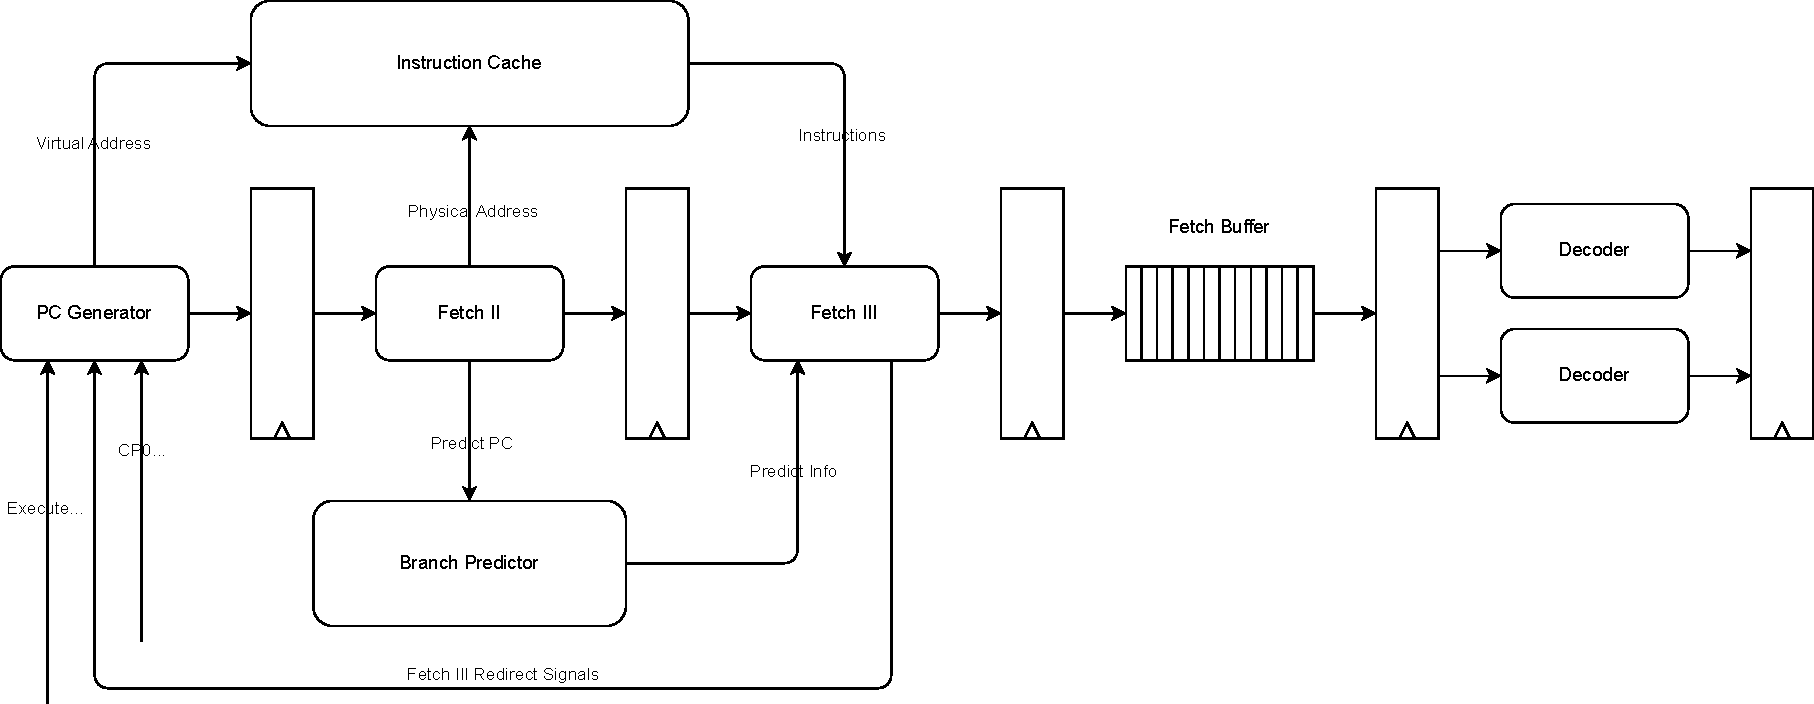
\includegraphics[width=\textwidth]{pic/front-end.pdf}
        \caption{前端架构设计简图}
    \end{figure}
\end{frame}

\begin{frame}
    \frametitle{后端架构}
    \begin{figure}
        \centering
        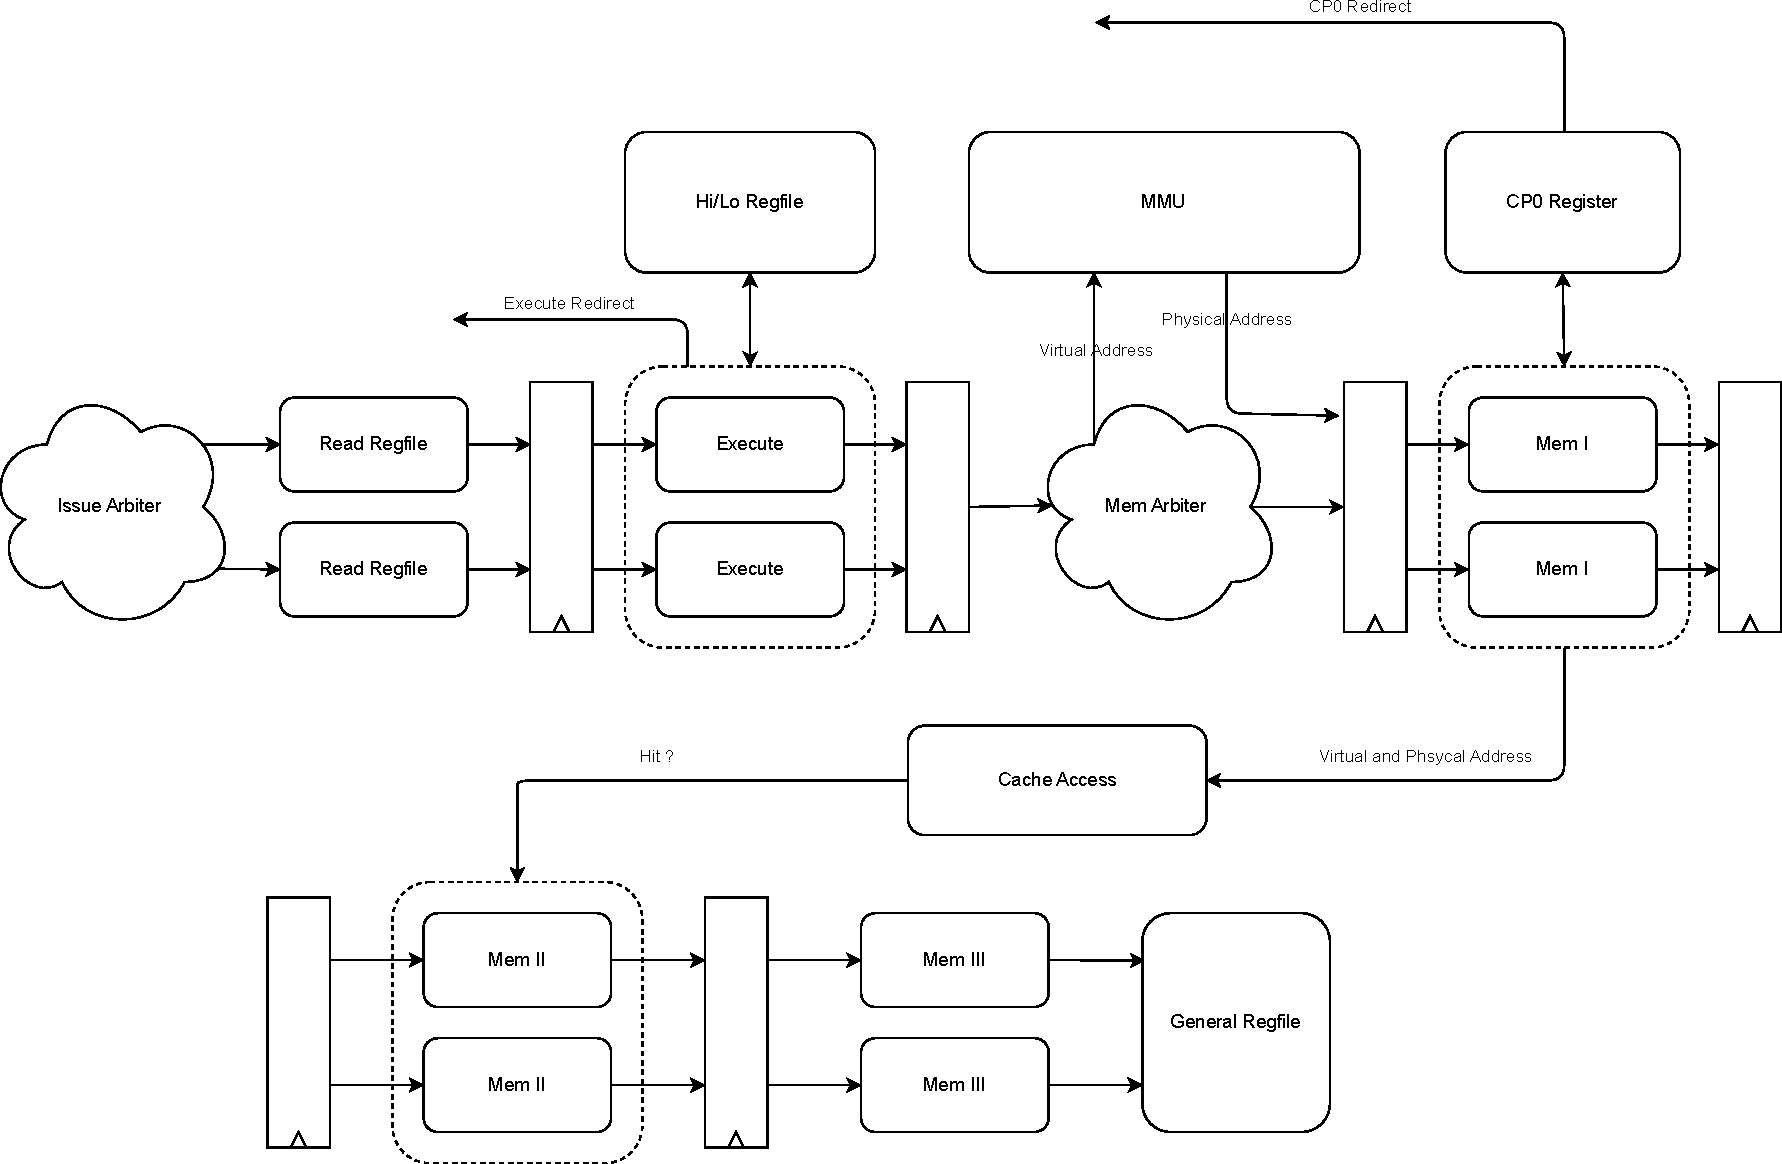
\includegraphics[width=0.9\textwidth]{pic/back-end.pdf}
        \caption{后端架构设计简图}
    \end{figure}
\end{frame}


\subsection{流水线设计}

\begin{frame}
    \frametitle{取指}
    \begin{itemize}
        \item 取指流水线\begin{itemize}
            \item Fetch 1: 仲裁PC,发送虚拟地址至ICache
            \item Fetch 2: 发送通过MMU获得的物理地址,若有异常,则作标记
            \item Fetch 3: 对ICache返回的指令作\textbf{分支快速译码},判断出分支指令,必要时进行PC重定向
        \end{itemize}
        \item 取指缓冲\begin{itemize}
            \item 16-Entries指针FIFO
            \item 每周期最多“4进2出”
            \item 跳过非分支延迟槽中的空指令
        \end{itemize}
        \item 分支预测\begin{itemize}
            \item RAS分支预测
            \item Bi--Mode分支预测器
            \item 256-Entries BTB
        \end{itemize}
    \end{itemize}
\end{frame}

\begin{frame}[fragile]
    \frametitle{取指缓冲对双访存的优化}
\begin{minipage}[c]{0.4\linewidth}
\begin{lstlisting}
sw t8, 0(a3)
lw t7, 8(t0)
nop
sw t7, 8(a3)
lw t6, 12(a0)
nop
sw t6, 12(a3)
lw t5, 16(a0)
nop
sw t4, 20(a3)
lw t3, 24(t0)
nop
...
\end{lstlisting}
    \end{minipage}\hfill
\begin{minipage}{0.4\linewidth}
\begin{lstlisting}
sw t8, 0(a3)
lw t7, 8(t0)

sw t7, 8(a3)
lw t6, 12(a0)

sw t6, 12(a3)
lw t5, 16(a0)

sw t4, 20(a3)
lw t3, 24(t0)

...
\end{lstlisting}
    
\end{minipage}
\end{frame}

\begin{frame}
    \frametitle{译码、发射与读寄存器}
    \begin{itemize}
        \item 译码\begin{itemize}
            \item 译码模块单独占一个流水级
            \item 将指令译成对应的uOp,并译出必要信息
            \item 判断是否为保留指令或会触发协处理器不可用的指令,并作标记
        \end{itemize}
        \item 发射\begin{itemize}
            \item 组合逻辑,与读寄存器共占一级流水级
            \item 进行单发射仲裁
        \end{itemize}
        \item 读寄存器\begin{itemize}
            \item 后续流水级旁路和通用寄存器堆间的数据仲裁
            \item 当所需数据在流水线中还没被计算出来时,暂停操作
            \item \textbf{提前计算跳转地址}供执行阶段进行分支预测正确性检验
        \end{itemize}
    \end{itemize}
\end{frame}

\begin{frame}
    \frametitle{执行}
    \begin{itemize}
        \item 执行\begin{itemize}
            \item 对于普通运算指令,执行阶段直接计算结果并放入流水线中
            \item 对于访存指令,执行阶段计算其访存地址\begin{itemize}
                \item 在初赛提交中,本周期还会进行访存地址冲突检查
                \item 在决赛提交中,访存地址冲突检查移到单独一级流水
            \end{itemize}
            \item 对于多周期指令,执行单元请求流水线暂停,直到其执行完毕
            \item 执行单元直接和Hi/Lo寄存器交互,故不需要对Hi/Lo寄存器作旁路转发
            \item 如果指令需要跳转,执行单元会发出跳转信号
        \end{itemize}
    \end{itemize}
\end{frame}

\begin{frame}[fragile]
    \frametitle{执行}
    \begin{minipage}[c]{0.23\linewidth}
        通过参数化标记,上下两个执行单元有着\textbf{不一样的功能,但用着同一份
        代码}。

        只有上执行单元拥有处理分支指令的能力,去除了无用的冗余,也不引来
        额外的麻烦。
    \end{minipage}
    \hfill\begin{minipage}{0.70\linewidth}
\begin{lstlisting}[language=scala]
class SingleExecute(
  advanced : Boolean = true
) extends Component {
  ...
}

class Execute extends Component {
  ...
  val units = Seq(
    new SingleExecute(true),
    new SingleExecute(false)
  )
  ...
}
\end{lstlisting}
    \end{minipage}
\end{frame}

\begin{frame}
    \frametitle{访存}
    \textbf{访存冲突与虚实转换流水级}:该级为决赛提交中拥有的一级流水级,原因在于
    决赛提交版本中含有TLB,访问需要较长的时间,因此我们对流水线再次进行了切分,其主要功能如下
    \begin{itemize}
        \item 地址冲突检查\begin{itemize}
            \item 若出现同时写同一个字对齐后的地址,则进行单发调度
            \item 若出现使用不同数据通路(DCache与Uncache)的地址,则进行单发调度
        \end{itemize}
        \item 虚实地址转换\begin{itemize}
            \item 访问TLB,获得VPN对应的PFN
            \item 若出现TLB异常,则对指令作标记,在下一周期中处理
        \end{itemize}
    \end{itemize}
\end{frame}

\begin{frame}
    \frametitle{访存}
    \begin{itemize}
        \item 访存第一阶段\begin{itemize}
            \item 向CacheAccess发送虚拟地址与物理地址,拉起访存请求
            \item 将指令的异常信息交付异常处理单元
        \end{itemize}
        \item 访存第二阶段\begin{itemize}
            \item 等待CacheAccess返回Hit信号
        \end{itemize}
        \item 访存第三阶段\begin{itemize}
            \item 收到返回的数据,写回通用寄存器堆
        \end{itemize}
    \end{itemize}
\end{frame}

\subsection{分支预测设计}

\begin{frame}
    \frametitle{Bi--Mode分支预测器}

    \begin{minipage}[c]{0.45\linewidth}
        % 在设计上,我们借鉴了开源的RISC-V处理器玄铁910的分支预测部分,采用了设计简单、
        % 性能优秀的Bi--Mode分支预测器。这种分支预测方法融合了局部分支预测和全局分支预测,
        % 充分利用了历史分支信息,同时还将倾向于跳转和倾向于不跳转的分支指令分两个表进行存储,
        % 有效降低了混叠干扰。
        \begin{itemize}
            \item 借鉴于\textbf{玄铁910}的分支预测设计
            \item \textbf{融全局与局部}为一体
            \item 分表存储,降低混叠
        \end{itemize}
    \end{minipage}\hfill
    \begin{minipage}{0.5\linewidth}
        \medskip
        \begin{figure}
            \centering
            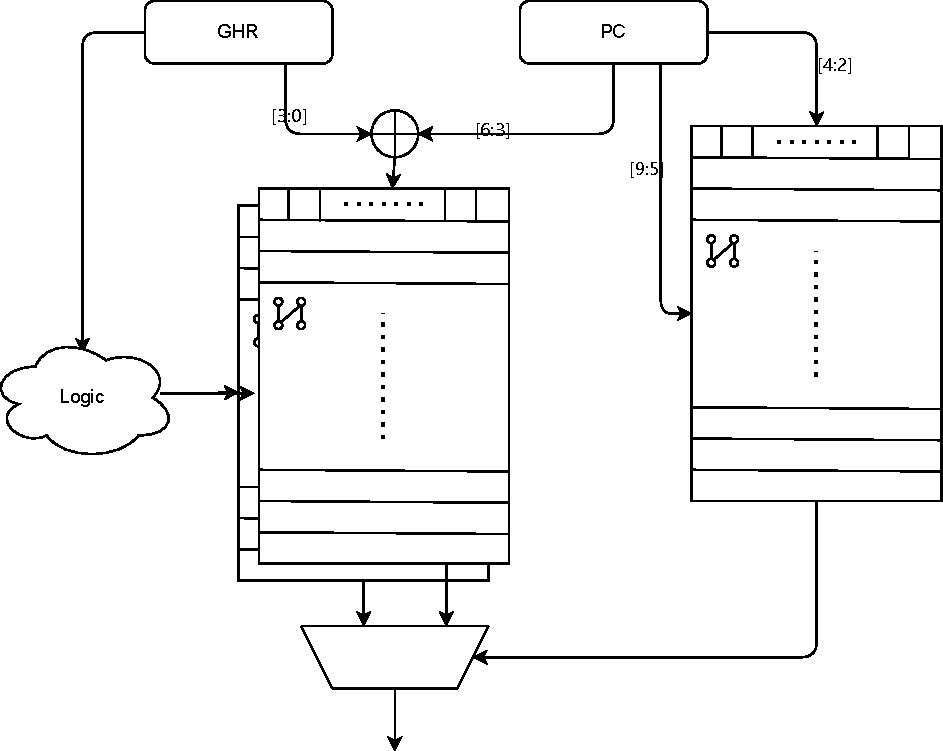
\includegraphics[width=\linewidth]{pic/branch-predict.pdf}
            \caption{分支预测图示}
        \end{figure}
    \end{minipage}

\end{frame}

\begin{frame}
    \frametitle{分支预测准确率}
    \begin{table}
        \centering
        \caption{性能测试中的分支预测表现}
        \begin{tabular}{lc|lc}
            \toprule
            程序 & 准确率 & 程序 & 准确率\\
            \midrule
            bubble sort & 70.1\% & coremark & 77.3\% \\
            crc32 & 95.3\% & dhrystone & 96.0\% \\
            quick sort & 75.5\% & select sort & 92.1\% \\
            sha & 97.6\% & stream copy & 97.1\% \\
            stringsearch & 88.4\% \\
            \bottomrule
        \end{tabular}
    \end{table}
\end{frame}

\subsection{高速缓存设计}

\subsubsection{指令高速缓存}

\begin{frame}
    \frametitle{指令高速缓存}

    \begin{itemize}
        \item 4路组相联
        \item 4 Banks
        \item 每周期可返回128 bit数据(4条指令)
        \item 取指合并\begin{itemize}
            \item 由于不能保证所需的4条指令在同一个缓存行中,因此每周期需要取
                  两条Cache Line
        \end{itemize}
    \end{itemize}

\end{frame}

\subsubsection{数据高速缓存}

\begin{frame}
    \frametitle{数据高速缓存}
\end{frame}

\section{系统设计}

\subsection{PMON}

\begin{frame}
    \frametitle{PMON}

    \begin{minipage}[c]{0.4\linewidth}
        成功启动PMON,并能正确运行PMON的全部指令
    \end{minipage}
    \hfill
    \begin{minipage}{0.5\linewidth}
        \begin{figure}
            \centering
            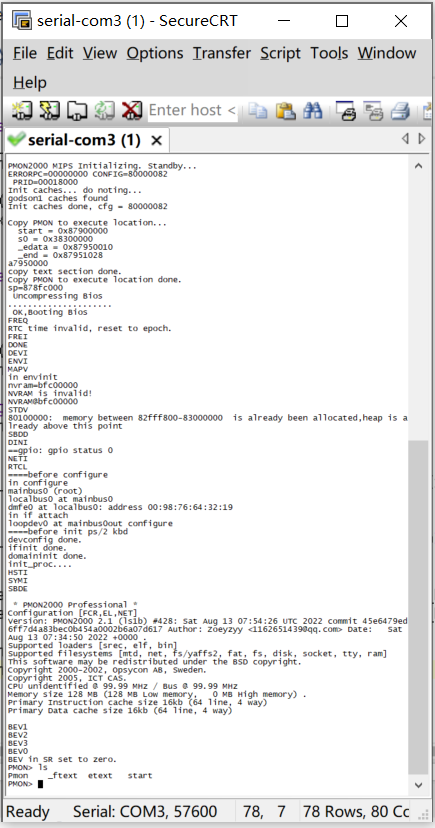
\includegraphics[width=0.7\textwidth]{pic/PMON.png}
        \end{figure}
    \end{minipage}

\end{frame}

\subsection{uCore}

\subsection{Linux}

\end{document}